\section{Chef}
\label{sec:chef}

Chef é uma ferramenta de gerenciamento e configuração de infraestrutura criada
pela comunidade Opscode em 2008 oficialmente lançada em 2009. Seu propósito é
tranformar uma infraestrutura complexa em código~\cite{chef:2016}. Sendo assim, a gerência de
configuração gira em torno da codificação simplificada e amigável
ao invés de comandos manuais de instalação e configuração de aplicações ~\cite{sharma:2015}.

A estrutura completa da ferramenta Chef contém vários componentes interagindo entre si para
prover ao cliente, ou seja, o ambiente alvo, as informações e instruções necessárias para que ele
possa executar sua função. Os principais componentes são~\cite{chefdoc:2016}:

\begin{itemize}
  \item \textit{Workstation}: qualquer máquina que possa servir como estação
    responsável por permitir usuários criar, testar e manter \textit{cookbooks};
  \item \textit{Cookbook}: contém as configurações desejadas para o ambiente.
    Pode ser customizados para um ambiente específico da empresa ou utilizar
    \textit{cookbooks} disponíveis pela comunidade Chef;
  \item \textit{Ruby}: linguagem oficial utilizada para a escrita dos \textit{scripts}
    é o Ruby;
  \item \textit{Node}: qualquer máquina física, virtual, em núvem, dispositivo
    de rede, etc, que deva ser gerenciada pelo Chef;
  \item \textit{Chef Client}: ferramenta instalada em todos os \textit{nodes}. O
    \textit{Chef Client} é responsável por executar todas as tarefas especificadas
    em uma \textit{run-list} (conjunto de \textit{cookbooks}). Esse componente é
    executado pela aplicação CLI \textit{chef-client};
  \item \textit{Chef Server}: funciona como um \textit{hub} de informações. Todos os
    \textit{cookbooks} e as políticas são atualizadas no Chef Server pelos usuários
    dos \textit{workstations}. O Chef Client acessa o Chef Server para verificar
    as informações necessárias para sua tarefas e retorna dados para o servidor
    que serão usados para gerar relatórios;
  \item \textit{Chef Analytics}: visibilidade em tempo real de dados informativos
    sobre o servidor como mudanças realizadas, os autores das mudanças e quando
    ocorreram. Além de detalhes das tarefas executadas nas máquinas \textit{nodes};
  \item \textit{Chef Supermarket}: local central onde a comunidade Chef cria e
    mantém os \textit{cookbooks}. Podem ser customizados de acordo com as necessidades
    da organização.
\end{itemize}

Desse componentes, tem-se os três principais: \textbf{Chef Server, Node} e \textbf{Workstation}.
A figura \ref{fig:chef-comp} mostra a relação entre esses três componente. Existem os requisitos
mínimos para a implementação do Chef~\cite{chefdoc:2016}:

\begin{itemize}
  \item As máquinas \textit{node} devem ter uma plataforma instalada (RedHat,
    Debian, OpenSUSE, etc);
  \item A maquina que contenha o Chef Server deve ter os requisitos
    mínimos de hardware especificada no site oficial do Chef;
  \item Todas as regras de rede e de \textit{firewall} devem estar configuradas
    corretamente.
\end{itemize}

\begin{figure}[H]
  \centering
  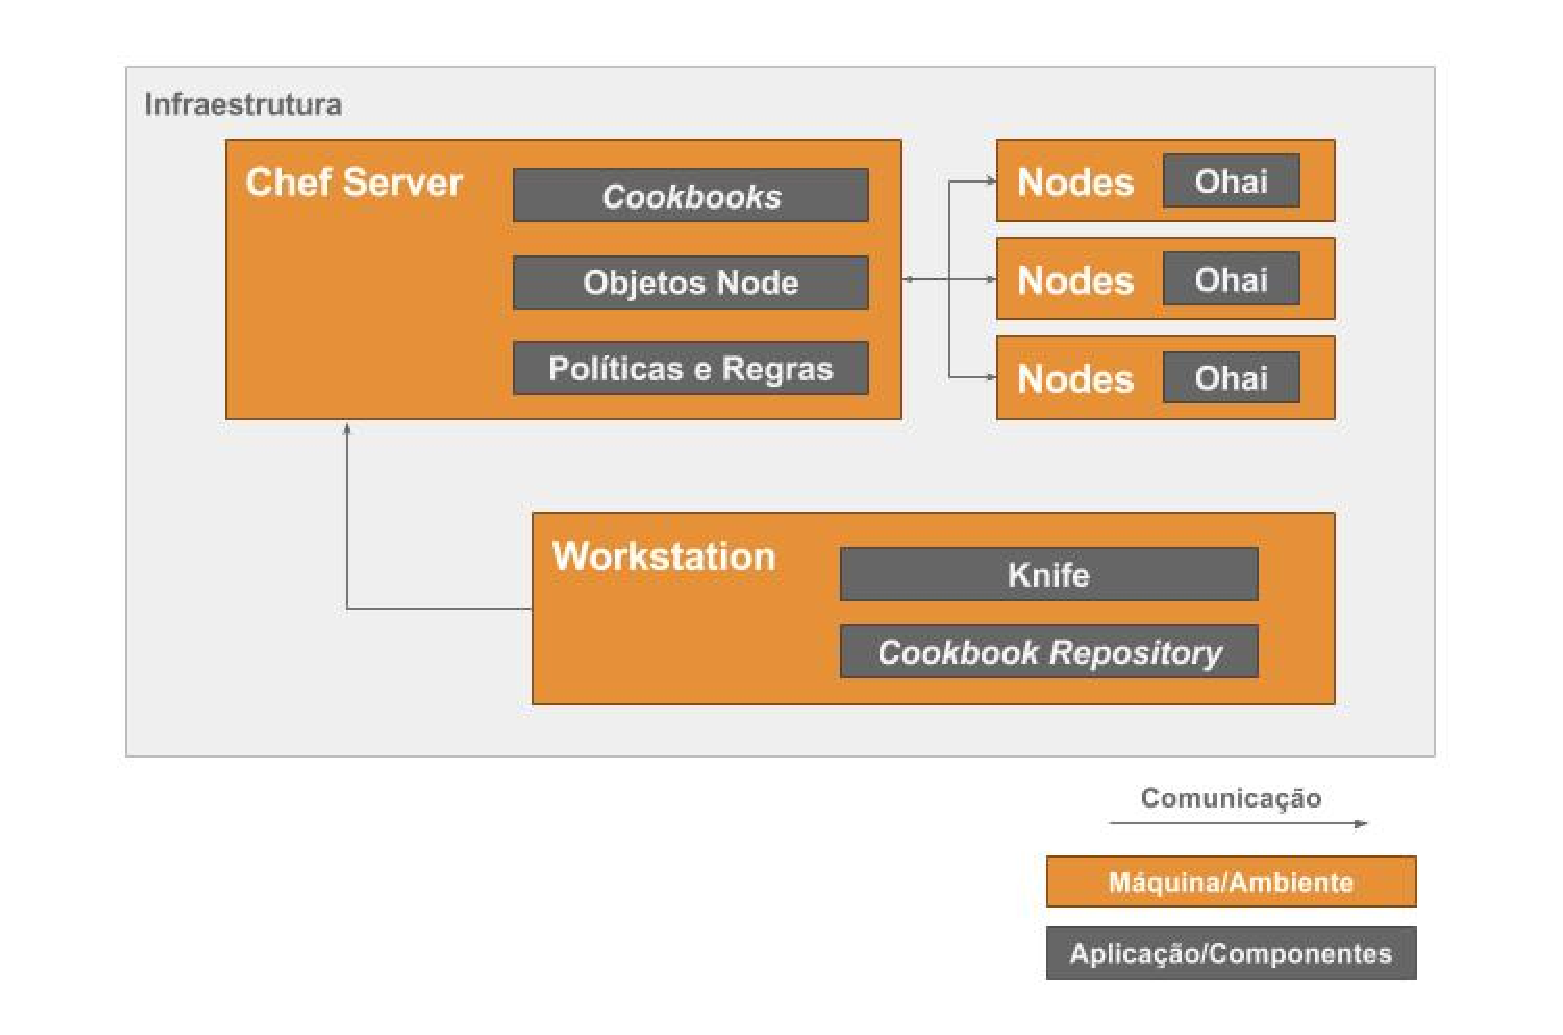
\includegraphics[width=0.8\textwidth]{figuras/chef-comp.eps}
  \caption{Relação entre os componente do Chef}
  \label{fig:chef-comp}
\end{figure}

\subsection{\textit{Cookbooks}}
\label{sec:chef-cookbooks}

\textit{Chef} utiliza os \textit{cookbooks} sendo a unidade básica de configuração do
ambiente. Neles são definidos comandos, arquivos, e outros atributos
para estabelecer o estado desejado para a instalação e configuração
do ambiente alvo \cite{sharma:2015}.

\citeonline{sharma:2015} Classifica os \textit{cookbooks} em três categorias:
\begin{itemize}
  \item \textbf{Aplicação}: contém as configurações de acordo com a instalação de
    uma aplicação. Exemplo PostgreSQL, Apache, Nginx;
  \item \textbf{Biblioteca}: define recursos a serem utilizados por outros \textit{cookbooks}.
    Não é recomendado utilizado diretamente em um node;
  \item \textbf{\textit{Wrapper}}: são \textit{cookbooks} prontos construidos pela comunidade que podem
    ser alterados para que se adequem ao ambiente que será implantado.
\end{itemize}

O componente \textit{chef-client} irá executar as receitas (mais detalhes sobre receitas ou
\textit{recipes} na seção \ref{sec:lev-rec}) disponíveis nos \textit{cookbooks}
indicados pelo \textit{Chef Server} quando necessário, ou seja, se não houver
nenhuma mudança quanto as configurações do ambiente o \textit{chef-client} não irá
alterar nada, do contrário ele irá aplicar as configurações necessárias~\cite{chefdoc:2016}.




